%%
%% Automatically generated file from DocOnce source
%% (https://github.com/hplgit/doconce/)
%%
%%


%-------------------- begin preamble ----------------------

\documentclass[%
oneside,                 % oneside: electronic viewing, twoside: printing
final,                   % draft: marks overfull hboxes, figures with paths
10pt]{article}

\listfiles               %  print all files needed to compile this document

\usepackage{relsize,makeidx,color,setspace,amsmath,amsfonts,amssymb}
\usepackage[table]{xcolor}
\usepackage{bm,ltablex,microtype}

\usepackage[pdftex]{graphicx}

\usepackage{fancyvrb} % packages needed for verbatim environments

\usepackage[T1]{fontenc}
%\usepackage[latin1]{inputenc}
\usepackage{ucs}
\usepackage[utf8x]{inputenc}

\usepackage{lmodern}         % Latin Modern fonts derived from Computer Modern

% Hyperlinks in PDF:
\definecolor{linkcolor}{rgb}{0,0,0.4}
\usepackage{hyperref}
\hypersetup{
    breaklinks=true,
    colorlinks=true,
    linkcolor=linkcolor,
    urlcolor=linkcolor,
    citecolor=black,
    filecolor=black,
    %filecolor=blue,
    pdfmenubar=true,
    pdftoolbar=true,
    bookmarksdepth=3   % Uncomment (and tweak) for PDF bookmarks with more levels than the TOC
    }
%\hyperbaseurl{}   % hyperlinks are relative to this root

\setcounter{tocdepth}{2}  % levels in table of contents

% Tricks for having figures close to where they are defined:
% 1. define less restrictive rules for where to put figures
\setcounter{topnumber}{2}
\setcounter{bottomnumber}{2}
\setcounter{totalnumber}{4}
\renewcommand{\topfraction}{0.95}
\renewcommand{\bottomfraction}{0.95}
\renewcommand{\textfraction}{0}
\renewcommand{\floatpagefraction}{0.75}
% floatpagefraction must always be less than topfraction!
% 2. ensure all figures are flushed before next section
\usepackage[section]{placeins}
% 3. enable begin{figure}[H] (often leads to ugly pagebreaks)
%\usepackage{float}\restylefloat{figure}

% --- fancyhdr package for fancy headers ---
\usepackage{fancyhdr}
\fancyhf{} % sets both header and footer to nothing
\renewcommand{\headrulewidth}{0pt}
\fancyfoot[LE,RO]{\thepage}
% Ensure copyright on titlepage (article style) and chapter pages (book style)
\fancypagestyle{plain}{
  \fancyhf{}
  \fancyfoot[C]{{\footnotesize \copyright\ 1999-2021, "Computational Physics II FYS4411/FYS9411":"http://www.uio.no/studier/emner/matnat/fys/FYS4411/index-eng.html". Released under CC Attribution-NonCommercial 4.0 license}}
%  \renewcommand{\footrulewidth}{0mm}
  \renewcommand{\headrulewidth}{0mm}
}
% Ensure copyright on titlepages with \thispagestyle{empty}
\fancypagestyle{empty}{
  \fancyhf{}
  \fancyfoot[C]{{\footnotesize \copyright\ 1999-2021, "Computational Physics II FYS4411/FYS9411":"http://www.uio.no/studier/emner/matnat/fys/FYS4411/index-eng.html". Released under CC Attribution-NonCommercial 4.0 license}}
  \renewcommand{\footrulewidth}{0mm}
  \renewcommand{\headrulewidth}{0mm}
}

\pagestyle{fancy}


% prevent orhpans and widows
\clubpenalty = 10000
\widowpenalty = 10000

% --- end of standard preamble for documents ---


% insert custom LaTeX commands...

\raggedbottom
\makeindex
\usepackage[totoc]{idxlayout}   % for index in the toc
\usepackage[nottoc]{tocbibind}  % for references/bibliography in the toc

%-------------------- end preamble ----------------------

\begin{document}

% matching end for #ifdef PREAMBLE

\newcommand{\exercisesection}[1]{\subsection*{#1}}


% ------------------- main content ----------------------



% ----------------- title -------------------------

\thispagestyle{empty}

\begin{center}
{\LARGE\bf
\begin{spacing}{1.25}
Project 2, Quantum Machine Learning. Deadline June 1, Spring 2021
\end{spacing}
}
\end{center}

% ----------------- author(s) -------------------------

\begin{center}
{\bf \href{{http://www.uio.no/studier/emner/matnat/fys/FYS4411/index-eng.html}}{Computational Physics II FYS4411/FYS9411}}
\end{center}

    \begin{center}
% List of all institutions:
\centerline{{\small Department of Physics, University of Oslo, Norway}}
\end{center}
    
% ----------------- end author(s) -------------------------

% --- begin date ---
\begin{center}
Apr 17, 2021
\end{center}
% --- end date ---

\vspace{1cm}


\subsection*{Introduction}

Why do people care about "Quantum Machine Learning", or "Quantum Computing" in general? A common observation that motivates quantum computing,
although it does not tell the whole story, is the striking fact than quantum information of a quantum system is in a sense
larger than the classical information of a comparable classical system. In the case of
bits and qubits, $n$ classical bits allows you to store the value of $n$ boolean variables $a \in [0,1]$,
whereas you need $2^n$ amplitudes $\alpha \in \mathbb{C}$ to describe the state of $n$ quantum bits, or qubits.
In other words, the (Hilbert )space in which the qubits live in exponentially bigger than that of the classical
counterpart. In the context of parameterized quantum circuits, one may prepare a state in the exponentially
large Hilbert space by applying some simple quantum operations to a set qubits that are all initialized in the zero-state.



\vspace{6mm}

% inline figure
\centerline{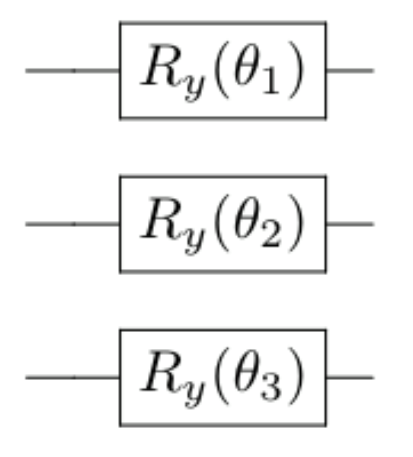
\includegraphics[width=0.6\linewidth]{figures/simple_ansatz.png}}

\vspace{6mm}




By varying $\theta_i \in [0, 2\pi]$, one can attain different states. A crucial thing to note is that we are not
able to prepare an arbitrary state using this ansatz as it much too constrained and simple: The exponentially large
space is not available to us. One might try to remedy this by introducing a more complex ansatz:



\vspace{6mm}

% inline figure
\centerline{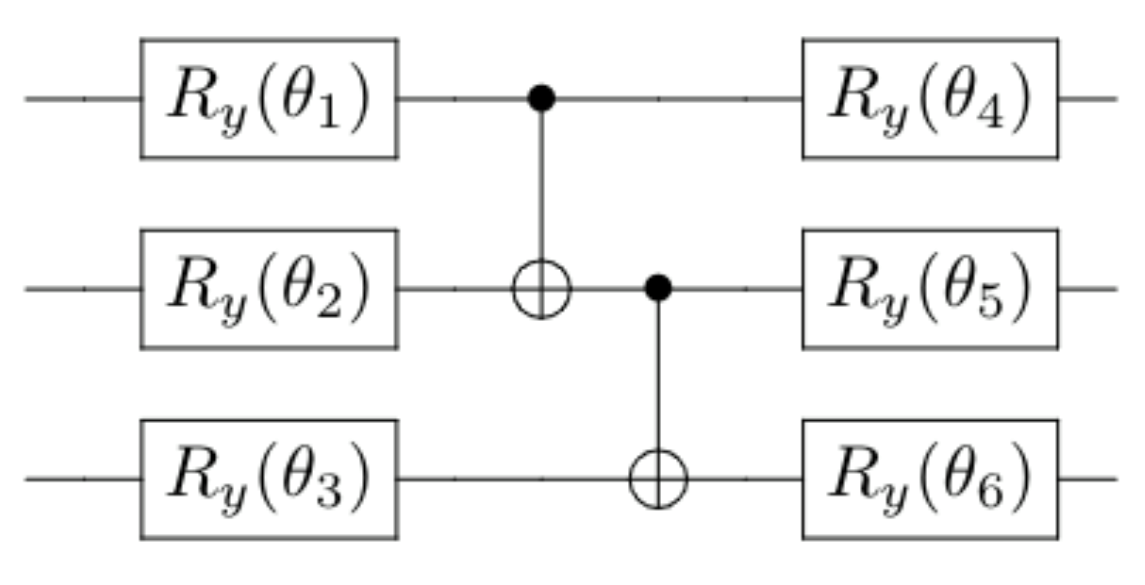
\includegraphics[width=1.0\linewidth]{figures/advanced_ansatz.png}}

\vspace{6mm}




We now have an ansatz whose number of operations scales polynomially in the number of qubits(in this case quadratic), and the
added complexity enables us to reach a greater part of Hilbert space. Still, it is only a polynomially large part of it, which
is vanishingly small compared to its full size. To have access to the whole space, one would in fact need to perform exponentially
many operations, which is practically intractable to do (Nielsen, 4.5.4).

Does this mean that the supposed power of quantum computation is practically inaccessible to us? No. Even though we
only reach a very small part of Hilbert space using "cheap" ansatzes, the states we do reach might be very useful
for solving a particular problem. Moreover, these states might be classically intractable to compute (source to come),
meaning the information they represent is not practical to determine using classical computers. They are however efficiently
prepared using quantum computers, as the number of quantum operations needed to be applied is by construction only polynomial.

How can one leverage this in a machine learning setting? A common approach is to use variants of the previous ansatzes to encode features to qubits by performing rotations, thus embedding the data in a high dimensional quantum state. Subsequent parameterized operations on the qubits then applies powerful transformations to the embedded data in a high dimensional space. Such methods are often described as quantum kernel methods, because of their similarity to classical kernel methods in machine learning.

For this project, you will perform quantum machine learning on the two first targets of Scikit learn iris data set. The data can be obtained the following way

\begin{print}
from sklearn import datasets
import numpy as np
iris = datasets.load_iris()
x = iris.data
y = iris.target
idx = np.where(y < 2) # we only take the first two targets.

x = x[idx,:]
y = y[idx]
\end{print}
$x$ is the feature matrix and $y$ are the targets.

\paragraph{Project 2 a): Encoding the Data Into a Quantum State.}
For this task you will consider a simple way of encoding a randomly generated data set sample into a quantum state:

\begin{print}
import qiskit as qk
import numpy as np
np.random.seed(42)

p = 2 #number of features
data_register = qk.QuantumRegister(p)
classical_register = qk.ClassicalRegister(1)

circuit = qk.QuantumCircuit(data_register, classical_register)

sample = np.random.uniform(size=p)
target = np.random.uniform(size=1)

for feature_idx in range(p):
    circuit.h(data_register[feature_idx])
    circuit.rz(2*np.pi*sample[feature_idx],data_register[feature_idx])

print(circuit)
\end{print}

The above code shows how a randomly generated data sample of $p=2$
features are encoded into a quantum state on two qubits utilizing
Qiskit. Each feature is encoded into a respective qubit utilizing a
$R_y(\theta)$ gate. The features are scaled with $2\pi$ to represent
rotation angles (the $R_y(\theta)$ gate performs a rotation). The
classical register will be used later for storing the measured value
of the circuit.  print(circuit) can be utilized at any point to see
what the circuit looks like.



Your task is to get familiar with the functionality utilized in the
above example and implement your own function to encode the
features of the iris data set to a quantum state.


\paragraph{Project 2 b): Processing the Encoded Data with Parameterized Gates.}
After the quantum state has been encoded with the information of a data set sample, one needs extend the circuit with operations that process the state in a way that allows us to infer the target data. This can be done by introducing quantum gates that are dependant on learnable parameters $\boldsymbol{\theta}$. We will do this in a similar fashion as for the encoding of the features:

\begin{print}
n_params = 4
theta = 2*np.pi*np.random.uniform(size=n_params)

circuit.ry(theta[0], data_register[0])
circuit.ry(theta[1], data_register[1])

circuit.cx(data_register[0], data_register[1])

circuit.ry(theta[2], data_register[0])
circuit.ry(theta[3], data_register[1])

circuit.cx(data_register[0], data_register[1])

print(circuit)
\end{print}

The above parameterization of the quantum state is what we will refer
to as the 'ansatz'. Your task is again to familiarize yourself with
the functionality utilized in the above example and implement your own
ansatz to be utilized together with the features of the
iris data set. The number of learnable parameters 'theta'
should be arbitrary.



\paragraph{Project 2c):Measuring the Quantum State and Making Inference.}
The next step is to generate a prediction from our quantum machine learning model. This is done by performing a measurement on the quantum state:

\begin{print}
circuit.measure(data_register[-1],classical_register[0])
shots=1000

job = qk.execute(circuit,
                backend=qk.Aer.get_backend('qasm_simulator'),
                shots=shots,
                seed_simulator=42
                )
results = job.result()
results = results.get_counts(circuit)

prediction = 0
for key,value in results.items():
    if key == '1':
        prediction += value
prediction/=shots
print('Prediction:',prediction,'Target:',target[0])
\end{print}
\begin{print}
    Prediction: 0.285 Target: 0.7319939418114051
\end{print}

In the above example, we are first applying a measurement operation on
the final qubit in the circuit, and we are interpreting our prediction
as the probability that this qubit is in the $\ket{1}$ state. Make
sure all the steps in the example are understood.

Implement your own function that generates a prediction by measuring one of the qubits.



\paragraph{Project 2d): Putting it all together.}
Now it is time to put together all of the above steps. Ideally, you
should make a class or a function that given a feature matrix of $n$
samples and an arbitrary number of model parameters, returns a vector
of $n$ outputs. For example:

\begin{print}
n = 100 #number of samples
p = 4 #number of features
theta = np.random.uniform(size=20) #array of model parameters
X = np.random.uniform(size=(n,p)) #design matrix
y_pred = model(X,theta) #prediction, shape (n)
\end{print}



We will now deal with how to train the model:

\paragraph{Project 2e): Parameter Shift-Rule and Calculating the Analytical Gradient.}
Since the model with random initial parameters is no good for
inference, we need to optimize the parameters in order to yield good
results, as is the usual with machine learning.

Since we are dealing with classification, we will use cross-entropy as the loss function

\begin{equation*}
    L = -\sum_{i=1}^{n}{y_i \ln{f(x_i;\boldsymbol{\theta})}},
\end{equation*}

where $y_i$ are the target labels, and
$f(\boldsymbol{x}_i;\boldsymbol{\theta})$ is the output of our model
for a given sample $\boldsymbol{x}_i$ and parameterization
$\boldsymbol{\theta})$. We calculate the gradiant by taking the
derivative of the loss with respect to the parameters

\begin{equation*}
    \frac{\partial}{\partial \boldsymbol{\theta}_k}L = \sum_{i=1}^{n}{\frac{f_i - y_i}{f_i(1 - f_i)}} \frac{\partial}{\partial \boldsymbol{\theta}_k}f_i,
\end{equation*}

where $f_i = f(x_i;\boldsymbol{\theta})$ for clarity. The only term we do not know how to calculate is $\frac{\partial}{\partial \boldsymbol{\theta}_k}f(x_i;\boldsymbol{\theta})$, but it turns out there is a simple trick to do this, the so-called parameter shift-rule \\cite{ParameterShift}. To calculate the derivative of the model output, we need to evaluate the model twice with the respective parameter shifted by a value $\frac{\pi}{2}$ up and down. The two resulting outputs are then put together to yield the derivative



\begin{equation*}
    \frac{\partial f(x_i; \theta_1, \theta_2, \dots, \theta_k)}{\partial \theta_j}  = \frac{f(x_i; \theta_1, \theta_2, \dots, \theta_j + \pi /2, \dots, \theta_k) -f(x_i; \theta_1, \theta_2, \dots, \theta_j - \pi /2, \dots, \theta_k)}{2}
\end{equation*}

Train your model by utilizing the Parameter Shift-Rule and some
gradient descent algorithm. Compare your results with for example
logistic regression.

Regular gradient descent does the job, but it is often outperformed by momentum based optimizers like Adam.


\paragraph{Project 2f): Adding Variations on the Data Encoding and Ansatz.}
Change/add more gates to the encoder and the parameterized ansatz to produce a more complex model (See for example figure 4 and figure 5 in \href{{https://arxiv.org/abs/2011.00027}}{\nolinkurl{https://arxiv.org/abs/2011.00027}} for inspiration). Train these new models on the iris data set. How do they compare? As a more challenging problem, you may train on the first few features of the Breast Cancer Data as well to see how the more powerful model performs.

\begin{print}
from sklearn.datasets import load_breast_cancer

data = load_breast_cancer()
x = data.data #features
y = data.target #targets
\end{print}





\subsection*{Introduction to numerical projects}

Here follows a brief recipe and recommendation on how to write a report for each
project.

\begin{itemize}
  \item Give a short description of the nature of the problem and the eventual  numerical methods you have used.

  \item Describe the algorithm you have used and/or developed. Here you may find it convenient to use pseudocoding. In many cases you can describe the algorithm in the program itself.

  \item Include the source code of your program. Comment your program properly.

  \item If possible, try to find analytic solutions, or known limits in order to test your program when developing the code.

  \item Include your results either in figure form or in a table. Remember to        label your results. All tables and figures should have relevant captions        and labels on the axes.

  \item Try to evaluate the reliabilty and numerical stability/precision of your results. If possible, include a qualitative and/or quantitative discussion of the numerical stability, eventual loss of precision etc.

  \item Try to give an interpretation of you results in your answers to  the problems.

  \item Critique: if possible include your comments and reflections about the  exercise, whether you felt you learnt something, ideas for improvements and  other thoughts you've made when solving the exercise. We wish to keep this course at the interactive level and your comments can help us improve it.

  \item Try to establish a practice where you log your work at the  computerlab. You may find such a logbook very handy at later stages in your work, especially when you don't properly remember  what a previous test version  of your program did. Here you could also record  the time spent on solving the exercise, various algorithms you may have tested or other topics which you feel worthy of mentioning.
\end{itemize}

\noindent
\subsection*{Format for electronic delivery of report and programs}

The preferred format for the report is a PDF file. You can also use DOC or postscript formats or as an ipython notebook file.  As programming language we prefer that you choose between C/C++, Fortran2008 or Python. The following prescription should be followed when preparing the report:

\begin{itemize}
  \item Use canvas to hand in your projects, log in  at  \href{{http://canvas.uio.no}}{\nolinkurl{http://canvas.uio.no}} with your normal UiO username and password.

  \item Upload \textbf{only} the report file!  For the source code file(s) you have developed please provide us with your link to your github domain.  The report file should include all of your discussions and a list of the codes you have developed.  The full version of the codes should be in your github repository.

  \item In your github repository, please include a folder which contains selected results. These can be in the form of output from your code for a selected set of runs and input parameters.

  \item Still in your github make a folder where you place your codes.

  \item In this and all later projects, you should include tests (for example unit tests) of your code(s).

  \item Comments  from us on your projects, approval or not, corrections to be made  etc can be found under your Devilry domain and are only visible to you and the teachers of the course.
\end{itemize}

\noindent
Finally,
we encourage you to work two and two together. Optimal working groups consist of
2-3 students. You can then hand in a common report.

% ------------------- end of main content ---------------

\end{document}

